\chapter{Numerical Implementation}
\label{chap:implementation}
\section{Coordinate Systems}
The ionosphere model that is presented in this paper is built in a spherical coordinate system. Spherical coordinates can be related to cartesian coordinates by the following equation:
\begin{equation}
	\bm r = \norm{\bm r}\left( \sin\theta\cos\phi, \sin\theta\sin\phi, \cos\theta\right)
	\label{eq:spherical_to_cartesian}
\end{equation}
There are two main benefits to using a spherical coordinate system for this problem. The first is the ability to use magnetic dipole coordinates as defined in~\citet{laundal2017}. This dipole coordinate system provides magnetic field orientation as a direct function of position, allowing the conductivity tensor that \citet{amm1996} presents (Equation~\ref{eq:conductivity_tensor}) to be utilized. The second is the ability to transform the coordinate system to geographic coordinates using a simple matrix rotation. This technique is discussed in~\citet{laundal2017}, and is required to calculate the relative sun-earth positions for extreme ultra violet (EUV) conductivity modeling.


\section{Discretization}
\label{sec:discretization}
Equation~\ref{eqn:continuity_eqn} can be combined with the conductivity tensor (Equation~\ref{eq:conductivity_tensor}) to produce Equation~\ref{eq:expanded_continuity_equation} as shown in~\citet{goodman1995} and~\citet{amm1996}. This provides a single equation relating the radial current to the ionospheric potential with coefficients containing the Hall, Pedersen and parallel conductivities in a spherical coordinate system.

\begin{equation}
	\begin{aligned}
		j_{R}(R_{E},\theta,\phi) & = \frac{1}{R_{E}^{2}} \Bigg[ \frac{\partial^{2}\psi}{\partial\theta^{2}} \frac{\Sigma_{0}\Sigma_{p}}{C}                                                                                                                                                                                             \\
		                         & \quad + \frac{\partial^{2}\psi}{\partial\phi^{2}} \left\{ \frac{1}{\sin^{2}\theta} \left( \Sigma_{p} + \frac{\Sigma_{H}^{2}\sin^{2}\epsilon}{C} \right) \right\}                                                                                                                                    \\
		                         & \quad + \frac{\partial\psi}{\partial\theta} \left\{ \frac{\partial}{\partial\theta} \left( \frac{\Sigma_{0}\Sigma_{p}}{C} \right) + \cot\theta\frac{\Sigma_{0}\Sigma_{p}}{C} + \frac{1}{\sin\theta}\frac{\partial}{\partial\phi} \left( \frac{\Sigma_{0}\Sigma_{H}\cos\epsilon}{C} \right) \right\} \\
		                         & \quad + \frac{\partial\psi}{\partial\phi} \left\{ \frac{\partial}{\partial\theta} \left( \frac{\Sigma_{0}\Sigma_{H}(-\cos\epsilon)}{C\sin\theta} \right) + \frac{1}{\sin^{2}\theta}\frac{\partial}{\partial\phi} \left( \Sigma_{p} + \frac{\Sigma_{H}^{2}\sin^{2}\epsilon}{C} \right) \right.       \\
		                         & \quad \left. + \frac{\Sigma_{0}\Sigma_{H}(-\cos\epsilon)\cot\theta}{C\sin\theta} \right\} \Bigg]_{R=R_{E}}
	\end{aligned}
	\label{eq:expanded_continuity_equation}
\end{equation}

For the majority of the points on the mesh, central-difference derivative discretizations were used as given in Equations~\ref{eq:first_order_discretization}~and~\ref{eq:second_order_discretization} (adapted to $\phi$ and $\theta$ from~\citet{William_H_Press1992-ps}).

\begin{align}
	\pdv{\psi}{\phi}(\theta,\phi) \approx \frac{\psi(\theta, \phi + \Delta\phi)- \psi(\theta, \phi - \Delta\phi)}{2\Delta \phi} &  & \pdv{\psi}{\theta} \approx \frac{\psi(\theta+ \Delta\theta,\phi)- \psi(\theta- \Delta\theta,\phi)}{2\Delta \theta}
	\label{eq:first_order_discretization}
\end{align}
\begin{align}
	\pdv[2]{\psi}{\phi}(\theta,\phi) \approx
	\frac{\psi(\theta, \phi + \Delta\phi) - 2\psi(\theta,\phi) + \psi(\theta, \phi - \Delta\phi)}{\Delta\phi^{2}}
	 &  &
	\pdv[2]{\psi}{\theta}(\theta,\phi) \approx
	\frac{\psi(\theta + \Delta\theta, \phi) - 2\psi(\theta,\phi) + \psi(\theta - \Delta\theta, \phi)}{\Delta\theta^{2}}
	\label{eq:second_order_discretization}
\end{align}

Figure~\ref{diag:std_five_point} displays the behaviour of these  discretizations and the five point stencil that is generated for each point in the mesh. This is shown for an example point in the low latitude region.
\begin{figure}[htbp]
	\centering
	\includestandalone[width=0.7\textwidth]{diagrams/LowLatGrid}
	\caption{Standard five-point stencil on the spherical grid. Displays the finite-difference contributions from the $\phi$ and $\theta$ derivative used in the general interior case.}
	\label{diag:std_five_point}
\end{figure}

The coefficients that contain a derivative in Equation~\ref{eq:expanded_continuity_equation} were computed using the same finite-difference stencils from Equations~\ref{eq:first_order_discretization} and~\ref{eq:second_order_discretization}. Since the conductivity values are known for every grid point, derivative matrices $D_\phi$ and $D_\theta$ were defined that include the contributions from the surrounding points. By ordering the elements on the mesh with a flattened index $i$, these derivatives were computed as follows:
\begin{align*}
	\left[\pdv{}{\theta} \left(\frac{\Sigma_0\sigp}{C}\right)\right]^{(i)} = \sum_{j=0}^{n_{\phi}n_{\theta}-1} D_\theta^{(i,j)} \left(\frac{\Sigma_0\sigp}{C}\right)^{(j)}
\end{align*}

Through this process, all of the coefficients were determined for every point on the mesh, allowing a coupled system to be assembled in Trilinos~\citep{TrilinosPaper}. This system was then solved iteratively as shown in Section~\ref{sec:solver}. The remaining piece of the discretization is the treatment of the boundaries imposed by the spherical coordinate system.
\section{Boundary Conditions}
\label{sec:polar_boundary}
The currents through which the magnetosphere couples with the ionosphere travel along the earth's magnetic field lines. Due to the structure of the earth's magnetic field, these field-aligned currents primarily enter the ionosphere in the high-latitude region. The continuity and accuracy of the system in the high latitude region is therefore paramount to the accuracy of the coupling. There are three distinct problems that arise when solving this equation on a spherical mesh, all occurring in the polar regions.
\begin{enumerate}
	\item In a standard spherical 2D mesh utilizing a $(\theta,\phi)$ coordinate system, a coordinate singularity naturally occurs at the poles as multiple $\phi$ values are mapped to the same point in physical space.
	\item The expanded continuity equation (Equation~\ref{eq:expanded_continuity_equation}) introduces terms of $\frac{1}{\sin\theta}$ that will approach infinity as the pole is approached. The coefficients overall do not diverge in the high latitude limit due to contributions from other terms, however the equation that describes the poles must take into account the numerical error that would be introduced by evaluating these $\sin\theta$ values at the poles. This can be done by either using a version of the equation that eliminates these terms in the polar limit or by not evaluating this equation at the poles entirely.
	\item The five-point finite-difference approximation breaks down as continuity over the pole requires the pole to calculate contributions from the surrounding ring of points of the pole, not just four adjacent points.
\end{enumerate}
Due to these issues, a more complex boundary condition is required at the poles. The implemented boundary condition leveraged the 2D divergence theorem to generate a finite-volume style stencil for the polar point. This is detailed in the next section.

\subsection{Polar Cap Finite-Volume Boundary Condition}
To determine an accurate potential at the pole, there must be continuity of the potential when approaching from any direction. It follows that any equation that relates the pole potential to the surrounding region must take into account all of the adjacent grid points shown in Figure~\ref{diag:pole_behaviour_grid}.

\begin{figure}[htbp]
	\centering
	\begin{subfigure}[t]{0.48\textwidth}
		\centering
		\includestandalone[width=\textwidth]{diagrams/CapBC1}
		\caption{Pole point and adjacent grid points.}
		\label{diag:pole_behaviour_grid}
	\end{subfigure}
	\hfill
	\begin{subfigure}[t]{0.48\textwidth}
		\centering
		\includestandalone[width=\textwidth]{diagrams/CapBC2}
		\caption{Pole cap region $\C$ and its boundary $\parC$ indicated on the grid.}
		\label{diag:pole_behaviour_grid_cap}
	\end{subfigure}
	\caption{Grid structure in the polar region. The polar cap region $\C$ is introduced at radius $\Delta\theta/2$ to apply an accurate boundary condition.}
\end{figure}

The polar divergence theorem boundary condition achieves this through defining a region of radius $\Delta\theta/2$ around the pole and then applying the divergence theorem to Equation~\ref{eqn:continuity_eqn} converting the expression to a line integral around the pole. Figure~\ref{diag:pole_behaviour_grid_cap} displays this region. This equation relates the values on the boundary $\parC$ to the total radial current passing through the $\C$ region as shown in Equation~\ref{eq:pole_integration_line2}.
\begin{equation}
	\iint_{\C} j_R(R_e) dA  =\iint_{\C}  \left[\nabla_\perp\cdot (\Sigma\cdot \nabla \psi)_\perp\right]dA
	\implies J_{cap}=\oint_{\parC}\left[(\Sigma\cdot \nabla \psi)_\perp\right]dl
	\label{eq:pole_integration_line2}
\end{equation}
$J_{\rm cap}$ provides the total current entering the region $\C$ in Figure~\ref{diag:pole_behaviour_grid_cap}. In practice, it is calculated by assuming that the polar current density $j_{R,pole}$ is representative of the average current density over the $\C$ region.
\begin{equation}
	J_{\rm cap} = j_{R,pole}\cdot A_\C = j_{R,pole}\cdot 2\pi R_E^2(1 -\cos\theta_{\parC})
\end{equation}
By evaluating the inner $\Sigma \cdot \nabla \psi$ expression in Equation~\ref{eq:pole_integration_line2} with the conductivity tensor in spherical coordinates and simplifying, Equation~\ref{eq:pole_integration_exp} is produced.
\begin{equation}
	J_{\rm cap} = \int_{0}^{2\pi}\left[\sin\theta_{\parC}\cdot
		\frac{\partial \psi}{\partial \theta}(\theta_{\parC}, \phi)\cdot
		\Sigma_{\theta\theta} (\theta_{\parC},\phi)\pm
		\frac{\partial\psi}{\partial\phi}(\theta_{\parC},\phi)\cdot
		\Sigma_{\theta\phi}(\theta_{\parC},\phi)
		\right] d\phi
	\label{eq:pole_integration_exp}
\end{equation}

Where $\theta_{\parC}=\Delta\theta/2$ and $\theta_0=\pi -\Delta\theta/2$ on the north and south pole respectively. The central sum is positive on the north pole and negative on the south pole due to the opposite direction of the normal vector to $\parC$ relative to $\hat\theta$ in the north and south poles.

\subsubsection{Discretization}
In this section a superscript of $(i,j)$ denotes evaluation at the grid point located at $(\theta_i,\phi_j)$. $(a,i)$ is used to denote evaluation on the adjacent points to the north pole as shown in Figure~\ref{diag:pole_behaviour_grid} for longitude $\phi_i$. $(\parC, i)$ is used to denote evaluation for a grid point on the polar cap boundary $\parC$ with the longitude $\phi_i$. The rest of the derivation will assume the north pole case with a positive normal.


To determine a linear representation of Equation~\ref{eq:pole_integration_exp} the first step involves discretizing the term obtained by the divergence theorem using a Riemann sum approximation, providing Equation~\ref{eq:fully_disc_pole}.
\begin{equation}
	J_{\rm cap} \approx\sum_{i=0}^{n_{\phi}-1}
	\left[
		\sin\theta_{\parC} \cdot \Sigma_{\theta\theta}^ {(\parC,i)}\cdot\frac{\partial \psi}{\partial \theta}^{(\parC,i)}+
		\Sigma_{\theta\phi}^{(\parC,i)}\cdot\frac{\partial\psi}{\partial\phi}^{(\parC,i)}
		\right] \Delta\phi
	\label{eq:fully_disc_pole}
\end{equation}
To create a linear equation containing the potential at the pole $\psi^{(\rm pole)}$ as a function of other grid points, the terms that are on $\parC$ must be eliminated from the equation. The $\theta$ derivative term is discretized using the standard first-derivative discretization with a denominator of $\Delta\theta$ due to $\parC$ being only $\Delta\theta/2$ from the pole (Equation~\ref{eq:first_order_discretization}). This introduces the pole into the equation and removes terms on the boundary $\parC$.
\begin{equation}
	\frac{\partial \psi}{\partial \theta}^{(\parC,i)}
	\approx \frac{\psi^{(\rm pole)} - \psi^{(a, i)}}{\Delta \theta}
\end{equation}
The discretized expansion can not be applied however to the $\phi$ derivative, since this would not remove the points on the boundary $\parC$. Therefore a different approach is required. The $\pdv{\psi}{\phi}$ term can be expanded into a Cartesian coordinate system by first applying the multi-variable chain rule.
\begin{equation*}
	\pdv{\psi}{\phi} =
	\pdv{\psi}{x}\pdv{x}{\phi}
	+ \pdv{\psi}{y}\pdv{y}{\phi}
	+\pdv{\psi}{z}\pdv{z}{\phi} = \bm\nabla \psi \cdot \pdv{\bm r}{\phi}
\end{equation*}
The $\hat\phi$ unit vector's direction can be determined with the following equation:
\begin{equation}
	\hat\phi = \left(-\sin\phi, \cos\phi, 0\right)
	\label{eq:phi_unit_vector}
\end{equation}
The $\pdv{\bm r}{\phi}$ term can be expanded by applying the spherical to Cartesian coordinate transformation Equation~\ref{eq:spherical_to_cartesian} for the mesh's radius of $R_E$ and applying the $\phi$ unit vector definition (Equation~\ref{eq:phi_unit_vector}) to simplify.
\begin{equation*}
	\pdv{\bm r}{\phi} = R_E\pdv{\phi} \left( \sin\theta\cos\phi, \sin\theta\sin\phi, \cos\theta\right) = R_E\sin\theta\left( -\sin\phi, \cos\phi,0 \right) = R_E\sin\theta\hat\phi
\end{equation*}
This provides the following expression for the $\phi$ derivative.
\begin{equation*}
	\pdv{\psi}{\phi} = \bm\nabla\psi \cdot R_E\sin\theta\hat\phi
\end{equation*}
Since $||\hat\phi|| = 1$ by definition, by the Cauchy–Schwarz inequality, $|\bm\nabla\psi \cdot \hat\phi| \le ||\bm\nabla\psi||\cdot  ||\hat\phi||= \norm{\bm\nabla\psi}$ which provides an upper bound on the absolute value of $\pdv{\psi}{\phi}$.
\begin{equation*}
	\abs{\pdv{\psi}{\phi}} = \abs{R_E\sin\theta (\bm\nabla\psi\cdot\hat\phi)}=\abs{R_E\sin\theta}\cdot \abs{\bm\nabla\psi\cdot \hat\phi} \le \abs{R_E\sin\theta}\cdot \norm{\bm\nabla\psi}
\end{equation*}
For a continuous electric field, the norm $\norm{\bm\nabla\psi}$ must be finite across all of the points on the mesh. Therefore it follows that in the limit of $\theta\rightarrow0$, the $\sin\theta$ term dominates resulting in the following expression.
\begin{equation*}
	\lim_{\theta\rightarrow0}\left|\pdv{\psi}{\phi}\right| = \lim_{\theta\rightarrow0} \left(\abs{R_E\sin\theta}\cdot \norm{\bm\nabla\psi}\right) = 0
\end{equation*}
Therefore, it follows that the $\phi$ derivative must go from a generally nonzero value at the adjacent grid points $\theta_a$ to zero at the pole. To approximate the value of the derivative at the midpoint $\parC$ between these points, a linear interpolation is performed and the Equation~\ref{eq:first_order_discretization} first-derivative central-difference approximation was applied to the resulting term:
\begin{equation}
	\frac{\partial \psi}{\partial \phi}^{(\parC,i)}
	\approx \frac{1}{2}\left(\pdv{\psi}{\phi}^{(a, i)} + \pdv{\psi}{\phi}^{(\rm pole)} \right) = \frac12\pdv{\psi}{\phi}^{(a,i)}
	\approx \frac{\psi^{(a, i+1)} - \psi^{(a, i-1)}}{4\Delta \phi}
\end{equation}
By performing a similar average on the conductivity values, a fully linear equation containing only points on the adjacent latitude ring and the pole itself can be obtained in Equation~\ref{eq:fully_disc_pole2}.

\begin{equation}
	\begin{aligned}
		J_{\rm cap} \approx\sum_{i=0}^{n_{\phi}-1}
		 & \left[
			\sin\theta_0\cdot
			\frac{\Sigma^{(a, i)}_{\theta\theta} + \Sigma^{(\rm pole)}_{\theta\theta}}{2}\cdot
			\frac{\psi^{(\rm pole)} - \psi^{(a, i)}}{\Delta \theta}\ +
		\right.                                                                                     \\
		 & \ \ \left.\frac{\Sigma^{(a, i)}_{\theta\phi} + \Sigma^{(\rm pole)}_{\theta\phi}}{2}\cdot
			\frac{\psi^{(a, i+1)} - \psi^{(a, i-1)}}{4\Delta \phi}
			\right] \Delta\phi
		\label{eq:fully_disc_pole2}
	\end{aligned}
\end{equation}
Equation~\ref{eq:fully_disc_pole2} provides a row in the linear system that couples the pole point to all of the $n_\phi$ adjacent points on the next latitude ring, maintaining continuity of the solution. Figure~\ref{fig:boundary_condition_contour} shows the behaviour of the potential solution from the ionosphere model at the pole, exhibiting continuous contour lines.

With the boundary condition, the linear system is complete. Section~\ref{sec:solver} describes the iterative methods used to solve the system.
\begin{figure}[H]
	\centering
	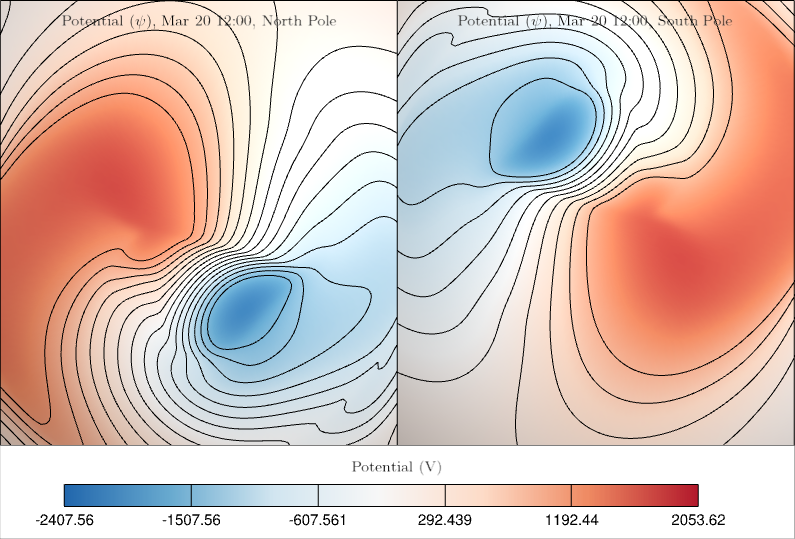
\includegraphics[width=0.7\textwidth]{figures/boundary condition zoomed.png}
	\caption{Boundary condition behaviour for an example southward interplanetary magnetic field solve showing continuous contour lines over the poles. }
	\label{fig:boundary_condition_contour}
\end{figure}

\section{Solver}\label{sec:solver}
In Sections~\ref{sec:discretization} and~\ref{sec:polar_boundary} a linear system of equations was produced to accurately model ionosphere electrodynamics for the magnetosphere-ionosphere coupling problem by solving Equation~\ref{eqn:continuity_eqn} on a 2D shell approximation of the ionosphere. In order to solve this system, the Trilinos~\citep{TrilinosPaper} C++ framework was used to build an MPI-parallel solver. This section will explore the different packages that were used and the implementation details of an iterative solve of this system.

\subsection{Trilinos Packages}
\subsubsection{Tpetra}
The coupled system that was generated from the combination of the five point stencil interior points and the polar divergence condition polar points was stored in Tpetra~\citep{TpetraPaper}. Tpetra provides a standard interface that allows a consistent representation for mathematical objects such as vectors and matrices in a wide array of modern Trilinos packages. Tpetra is also used to manage the distribution of vector and matrix elements between MPI ranks through a common interface known as a \texttt{Tpetra::Map}. This allows the ability to tweak the distribution on a global scale by changing a single \texttt{Tpetra::Map} instance. In this application, a sequential contiguous block of rows in $\phi$-major order was provided to each rank. However, potentially exploring different distribution strategies such as interleaved row storage between ranks or using the Zoltan~\citep{ZoltanUsersGuide} framework could potentially improve the performance of the application further and this is planned to be explored in the future.
\subsubsection{Belos}
Belos~\citep{BelosPaper} is an iterative solver library in Trilinos that provides a number of iterative solvers with configurable parameters. Belos provides a \texttt{Belos::SolverFactory} class that enables swapping solvers for performance analysis on the fly. A runtime analysis on the system was performed to determine the improved solver choice and configuration settings for this problem and this is detailed in Section~\ref{sec:convergence_study}. In the end a \texttt{GMRES} solver with preconditioning was used as this showed the highest performance on the matrix generated by this problem. The Belos solver and the associated solver parameters are configurable from a YAML configuration file that is passed into the application as a command line argument. This allows for easy solver and parameter performance studies and tuning without requiring re-compilation of the application.
\subsubsection{Preconditioning}
Two preconditioning strategies were explored in this problem. MueLu~\citep{MueLuUsersGuide} provides multi-grid preconditioning and solvers implemented using the Tpetra interface. IfPack2 is also included within the application and provides incomplete lower upper triangularization preconditioning methods. Similarly to the Belos solver, the preconditioner for the problem and its associated parameters are configurable through the YAML configuration file. This provides a single configuration file that can be used to tune the performance of the preconditioner for this problem. Section~\ref{sec:convergence_study} contains suggested values for the preconditioner that were found to be well performing through empirical testing.
\subsection{Application Structure}
\label{sec:application_structure}
The core of the configurability of this solver is the YAML configuration file that can be passed as a command line argument to the application. The boundary condition and equation can be configured through this file. While the current application only offers the use of the continuity equation Equation~\ref{eqn:continuity_eqn} from~\citet{goodman1995} with the conductivity tensor provided by~\citet{amm1996} combined with the boundary condition discussed in Section~\ref{sec:polar_boundary}, there are plans to extend these capabilities. Specifically, there is an alternative boundary condition that is in the process of implementation that utilizes a ``ghost ring'' approach to estimate the value at the pole using multiple five point stencils at a small distance from the pole and averages them. Additionally, incorporating the original conductivity tensor provided by~\citet{goodman1995} is also being explored as this will provide a conductivity tensor that does not require the approximation of the parallel conductivity as described in Chapter~\ref{chap:conductivity}.

\begin{figure}[htbp]
	\centering
	\includestandalone[width=\textwidth]{diagrams/SolverDiagram}
	\caption{Application structure diagram displaying the data flow of the solver and the configurable YAML parameters. Solid lines indicate the flow of computed parameters while the dashed lines display the configuration parameters. Conductivity tensor $\Sigma$ shows incoming data from the conductivity model described in Chapter~\ref{chap:conductivity}. The full application diagram is shown in Figure~\ref{diag:full_flow2}.}
	\label{diag:solver_flow}
\end{figure}
Figure~\ref{diag:solver_flow} displays the solver application structure from a high level view, and from this, the main solver loop can be clearly seen. The application will take in the interpolated MHD field aligned current data mapped down to the ionosphere; use that to generate the associated matrix, source term and initial guess based on the equation structure and boundary condition provided by the YAML file; then it will proceed to apply the preconditioner and solver to the problem, returning the potential to the MHD model to close the magnetospheric currents.

The MHD interpolation is currently in progress as indicated in Figure~\ref{diag:solver_flow} and therefore the figures in Chapter~\ref{chap:results} are generated using a pre-interpolated source term that was produced by the ionosphere model used in~\citet{global_groth_2000}. Once the coupling is complete, this circular loop structure will allow the application to run in parallel with the MHD code, receiving updated radial currents, over multiple MHD time-steps, piped into the application. This will allow the application to retain matrix structure through iterations. The feasibility of this is dependent on the timescale involved due to the conductivity being dependent on date and time, however this could potentially reduce the solve time as discussed in Section~\ref{sec:convergence_study}.

\section{Runtime Analysis and Solver Optimization}
\label{sec:convergence_study}
A short convergence speed study was performed on the model to determine parameters for the preconditioner and Belos solver to improve the performance. This was performed on a grid with size $n_\phi = 512$ and $n_\theta=256$. As discussed in Section~\ref{sec:solver}, both MueLu and IfPack2 preconditioners were tested to determine the best-performing configuration for the application. This was done in two stages. The first stage involved running the simulation on the same source input, testing different preconditioners and solvers while sweeping through their parameters. In the second stage, a convergence analysis was performed on the best resulting configuration for IfPack2 ILU preconditioning and the best resulting configuration with the MueLu preconditioning for a more comprehensive comparison.
\subsection{Parameter Sweep}
\label{sec:parameter_sweep}
For this stage of the experiment, two preconditioning packages were examined. The first using algebraic multi-grid provided by MueLu as a preconditioner with the \texttt{RILUK} solver used as a smoother and coarse solver, and the second using IfPack2 with \texttt{RILUK}. \texttt{RILUK} is the Trilinos implementation for ILU factorization. These preconditioners were found to have the best performance from the MueLu and Ifpack2 packages on this problem at default settings and therefore were selected for further testing. The \texttt{GMRES} solver from Belos was used as the solver for the problem and was chosen similarly as it was the Belos solver that produced the fastest runtime on this problem at default settings. Table~\ref{tab:sweep_riluk} shows the parameters that were tested for the IfPack2 ILU preconditioning and Table~\ref{tab:sweep_muelu} shows the parameters that were tested for the MueLu preconditioning. All tests were performed on a linux workstation with an \textbf{AMD Ryzen 5800x 8-core processor} with 16 threads available through simultaneous multithreading and 32GB of \textbf{DDR4 RAM}. Runtime was compared using the wall-clock runtime for the solver section of the application for one run of each of the configurations.
\begin{table}[H]
	\centering
	\begin{minipage}{0.48\textwidth}
		\centering
		\begin{tabular}{ll}
			\toprule
			\textbf{Parameter} & \textbf{Values}  \\
			\midrule
			Fill Level         & 2, 5, 10, 15, 20 \\
			Num Blocks         & 100, 200, 500    \\
			Processor Count    & 2, 4, 8, 14      \\
			\bottomrule
		\end{tabular}
		\captionof{table}{Ifpack2 RILUK sweep configurations}
		\label{tab:sweep_riluk}
	\end{minipage}
	\hfill
	\begin{minipage}{0.48\textwidth}
		\centering
		\begin{tabular}{ll}
			\toprule
			\textbf{Parameter}  & \textbf{Values} \\
			\midrule
			Smoother Fill Level & 1, 2, 4         \\
			Num Blocks          & 100, 200, 500   \\
			Processor Count     & 2, 4, 8, 14     \\
			\bottomrule
		\end{tabular}
		\captionof{table}{MueLu sweep configurations}
		\label{tab:sweep_muelu}
	\end{minipage}
\end{table}
This resulted in 60 configurations tested for the IfPack2 preconditioner and 24 for the MueLu preconditioner. The 14 processor runs were included in this analysis, however due to the simultaneous multi-threading on the CPU it is not possible to assign 14 physical cores to the problem. The runs for processor count of 14 are therefore likely not as indicative of scaling performance of this application. The raw results of this analysis are summarized in Tables~\ref{tab:ifpack_results} and \ref{tab:muelu_results} for the RILUK and MueLu preconditioners respectively. The fastest runtime for IfPack2 was achieved with 500 for num blocks in GMRES and a level of fill of 10 for ILUK on 8 processors. The best performing MueLu configuration was GMRES with a \texttt{num blocks} of 100 and a smoother fill level of 4 on 8 processors. These configurations were then selected for a more in depth convergence study as detailed in Section~\ref{sec:convergence_analysis}.
\subsection{Convergence Analysis}
\label{sec:convergence_analysis}
For the convergence analysis, the best performing algorithms from Section~\ref{sec:parameter_sweep} were run 10 times each on 2, 4, 8 and 14 processors. Multiple metrics were tracked throughout the simulation including the wall-clock time for conductivity computation and solver setup and computation. Additionally the iteration counts were recorded as well as the relative residual per iteration. Figures~\ref{fig:scaling_time} and~\ref{fig:scaling_iters} display the scaling behaviour of the algorithm iteration count and solve time (wall clock time between starting preconditioner setup and solver completion).
\begin{figure}[ht]
	\centering
	\begin{subfigure}[t]{0.45\textwidth}
		\centering
		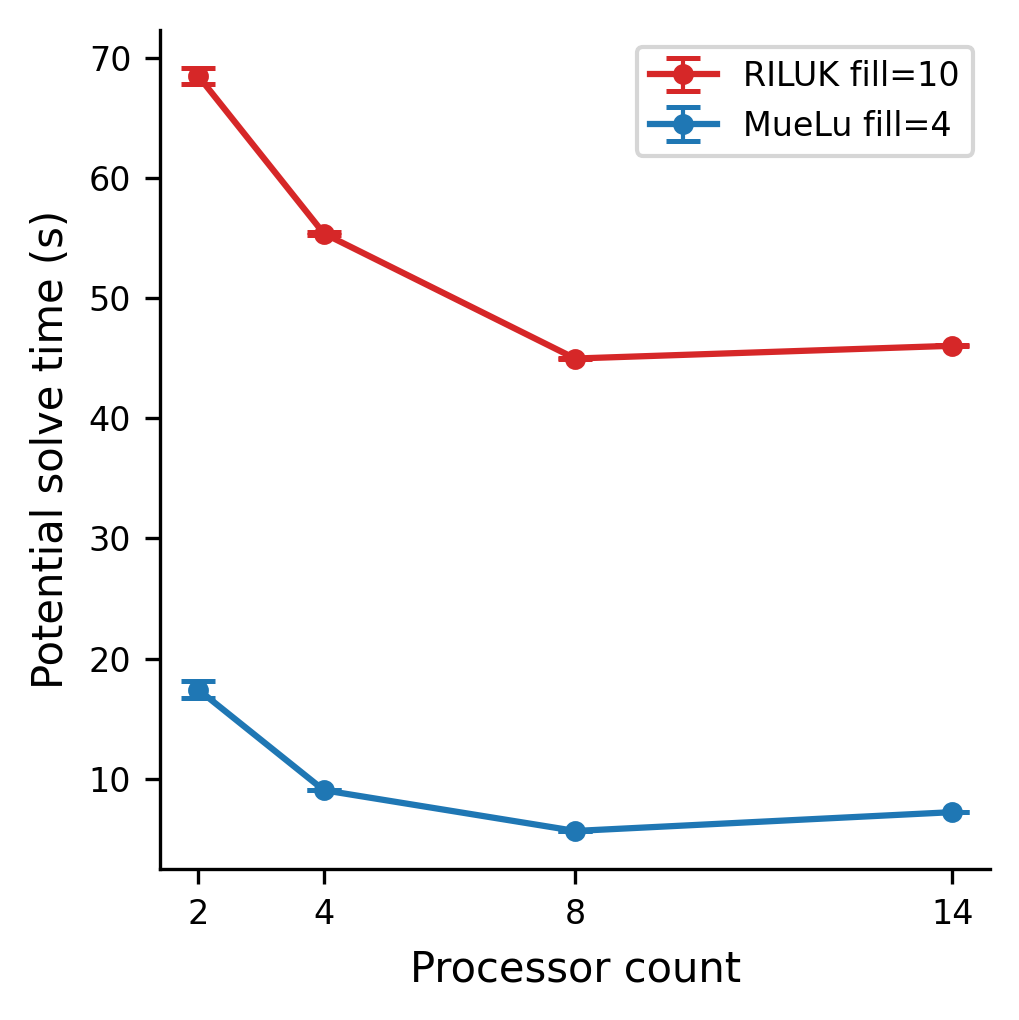
\includegraphics[width=\textwidth]
		{../convergenceAnalysis/plotsAndData/optimalRun/scaling_time_errorbars.png}
		\caption{Wall clock solve time for the coupled potential system for the MueLu and RILUK algorithms vs processor count.}
		\label{fig:scaling_time}
	\end{subfigure}
	\hfill
	\begin{subfigure}[t]{0.45\textwidth}
		\centering
		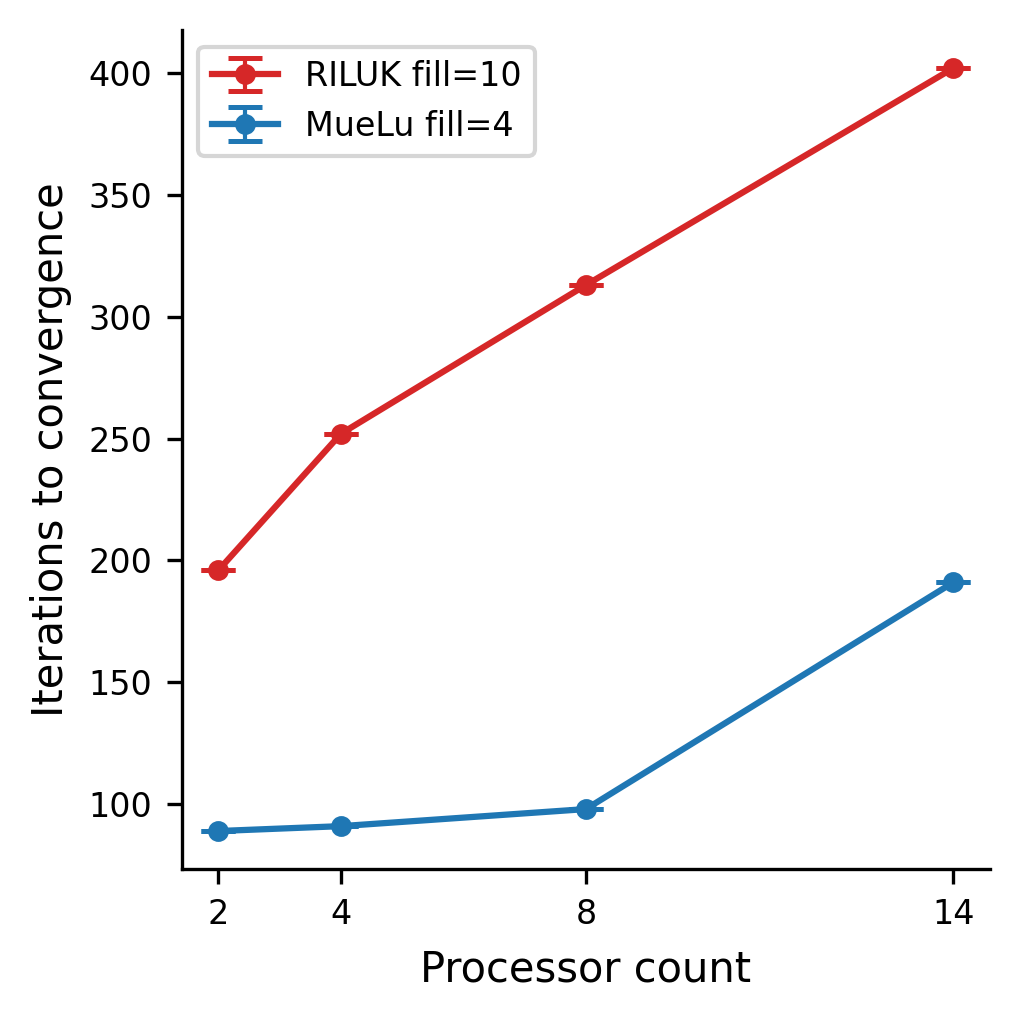
\includegraphics[width=\textwidth]
		{../convergenceAnalysis/plotsAndData/optimalRun/scaling_iterations_errorbars.png}
		\caption{Number of iterations to solve the coupled potential system for the MueLu and RILUK algorithms vs processor count.}
		\label{fig:scaling_iters}
	\end{subfigure}
	\caption{Application scaling behaviour for the IfPack2 and MueLu preconditioners across increasing processor counts, averaged over the 10 runs.}
	\label{fig:scaling_time_iters}
\end{figure}

Figure~\ref{fig:scaling_time} compares the wall-clock runtime for the two preconditioners. It can be clearly seen that the MueLu's algebraic multi-grid produced significantly faster results. Notably, the increase in performance from 2 to 4 processors is relatively significant, however the improvement from 4 to 8 is notably reduced, especially for the MueLu preconditioner. In both algorithms, the solve time of the 14 processor runs was slower than the 8 processor runs. This scaling behaviour could be due to increasing communication requirements between MPI ranks but more comprehensive testing on a dedicated network with more than 8 cores would be required to verify this. Figure~\ref{fig:scaling_iters} shows the iteration count required to reach the $1\times10^{-6}$ relative residual target. The IfPack2 preconditioner showed a rapid increase in iteration count from 2 to 14 processors, whereas the MueLu iteration count remained much more stable between 2 and 8 processors, only increasing in the 14 processor case.

Figure~\ref{fig:scaling_wallclock} shows the total runtime of both preconditioner configurations. It shows a similar trend to the results shown in the figures in~\ref{fig:scaling_time_iters}. This shows the minimal effect that the conductivity overhead has on the application runtime.
\begin{figure}[H]
	\centering
	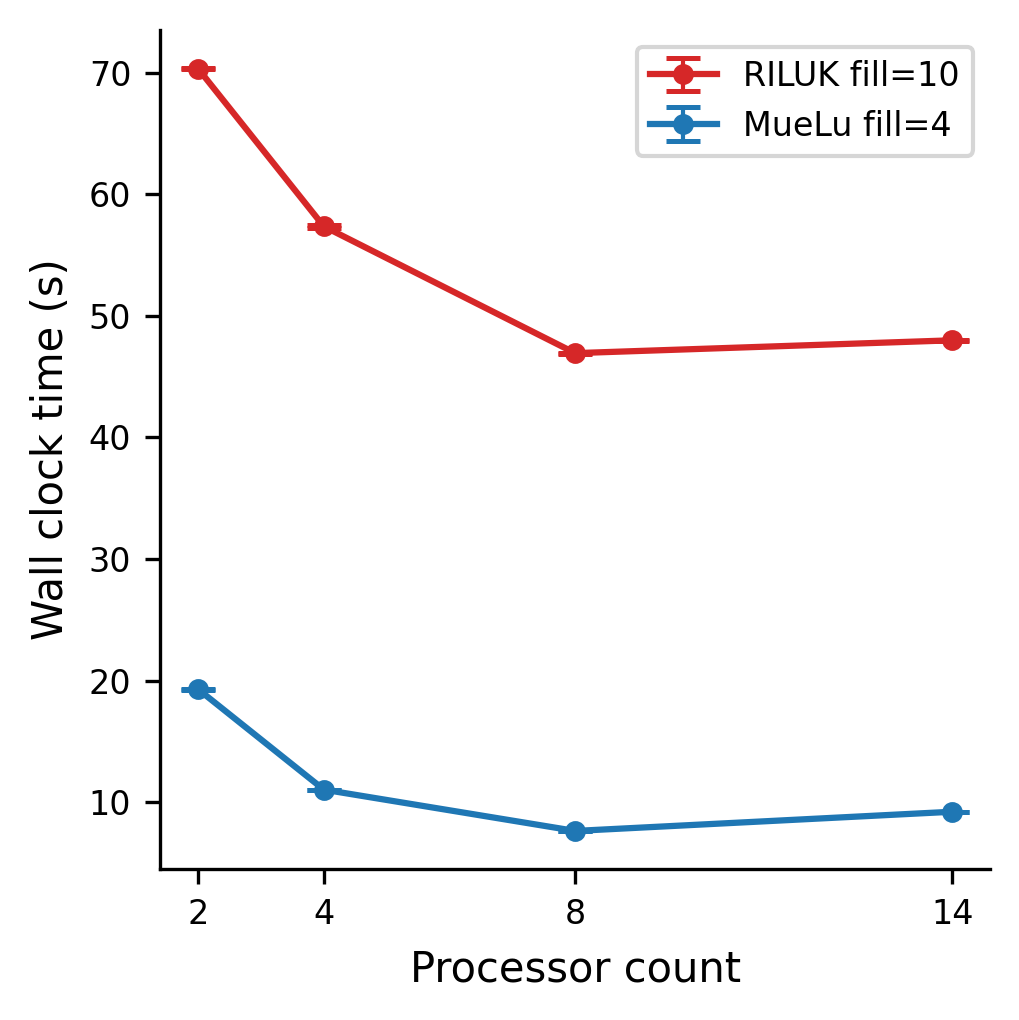
\includegraphics[width=0.45\textwidth]
	{../convergenceAnalysis/plotsAndData/optimalRun/scaling_wallclock_errorbars.png}
	\caption{Total wall clock time for the application solve portion for the IfPack2 and MueLu preconditioners vs processor count averaged over the 10 runs.}\label{fig:scaling_wallclock}
\end{figure}


\begin{figure}[ht]
	\centering
	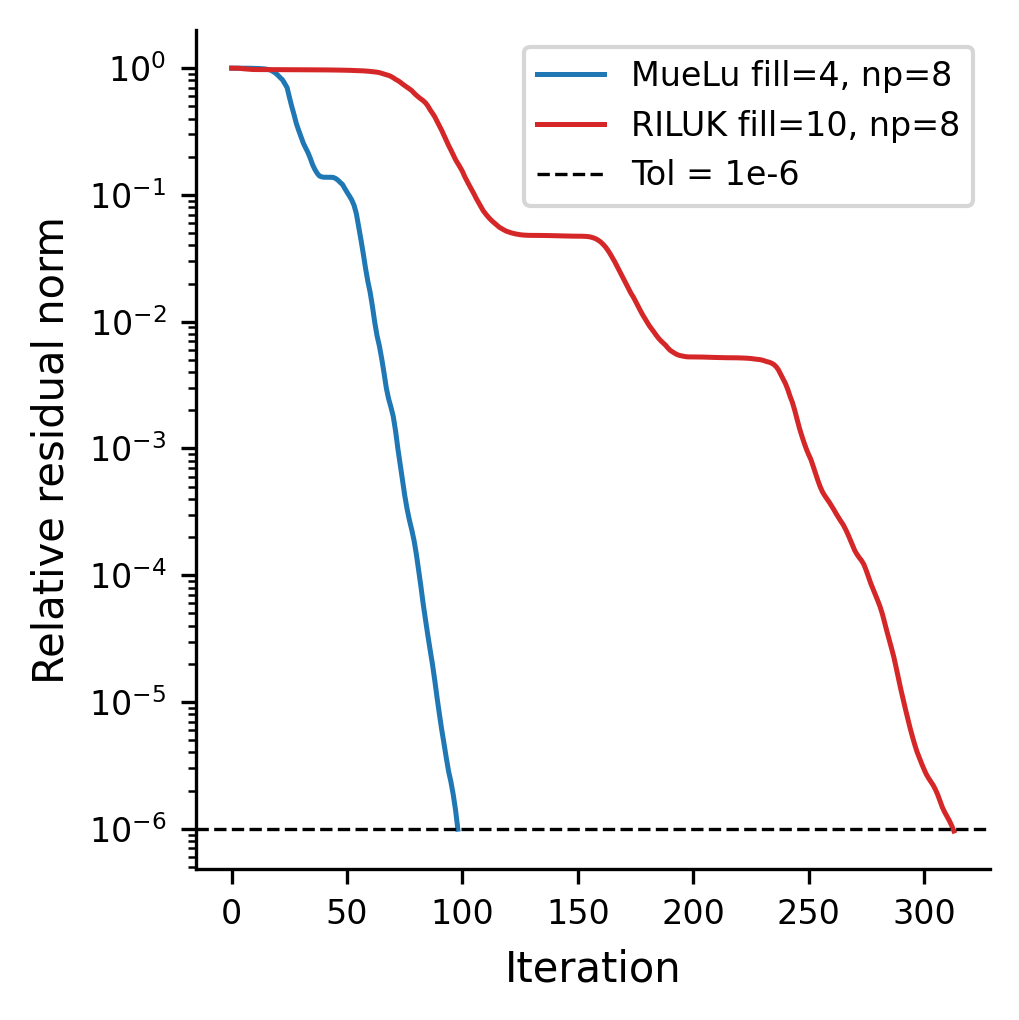
\includegraphics[width=0.45\textwidth]
	{../convergenceAnalysis/plotsAndData/optimalRun/convergence_curves.png}
	\caption{Convergence plot for the IfPack2 (\texttt{RILUK}) preconditioner vs the MueLu preconditioner. Shows relative residual (logarithmic) vs iteration count with the $1\times10^{-6}$ convergence tolerance displayed. Averaged over the 10 runs.}
	\label{fig:convergence_curves}
\end{figure}
In Figure~\ref{fig:convergence_curves} the convergence behaviour of both preconditioners can be seen averaged over the 10 runs. The IfPack2 preconditioner showed clear stalling behaviour at multiple iteration levels which was clearly reduced with the MueLu preconditioner. Overall, the convergence behaviour of the MueLu preconditioner showed largely improved results over just using \texttt{RILUK} provided by IfPack2 on this problem.

Figure~\ref{fig:time_breakdown} displays the time breakdown between the different sections of the application averaged over the 10 runs of the application. This shows the significant portion of application runtime that is dedicated to the solve procedure itself and the importance of solver optimization.
\begin{figure}[H]
	\centering
	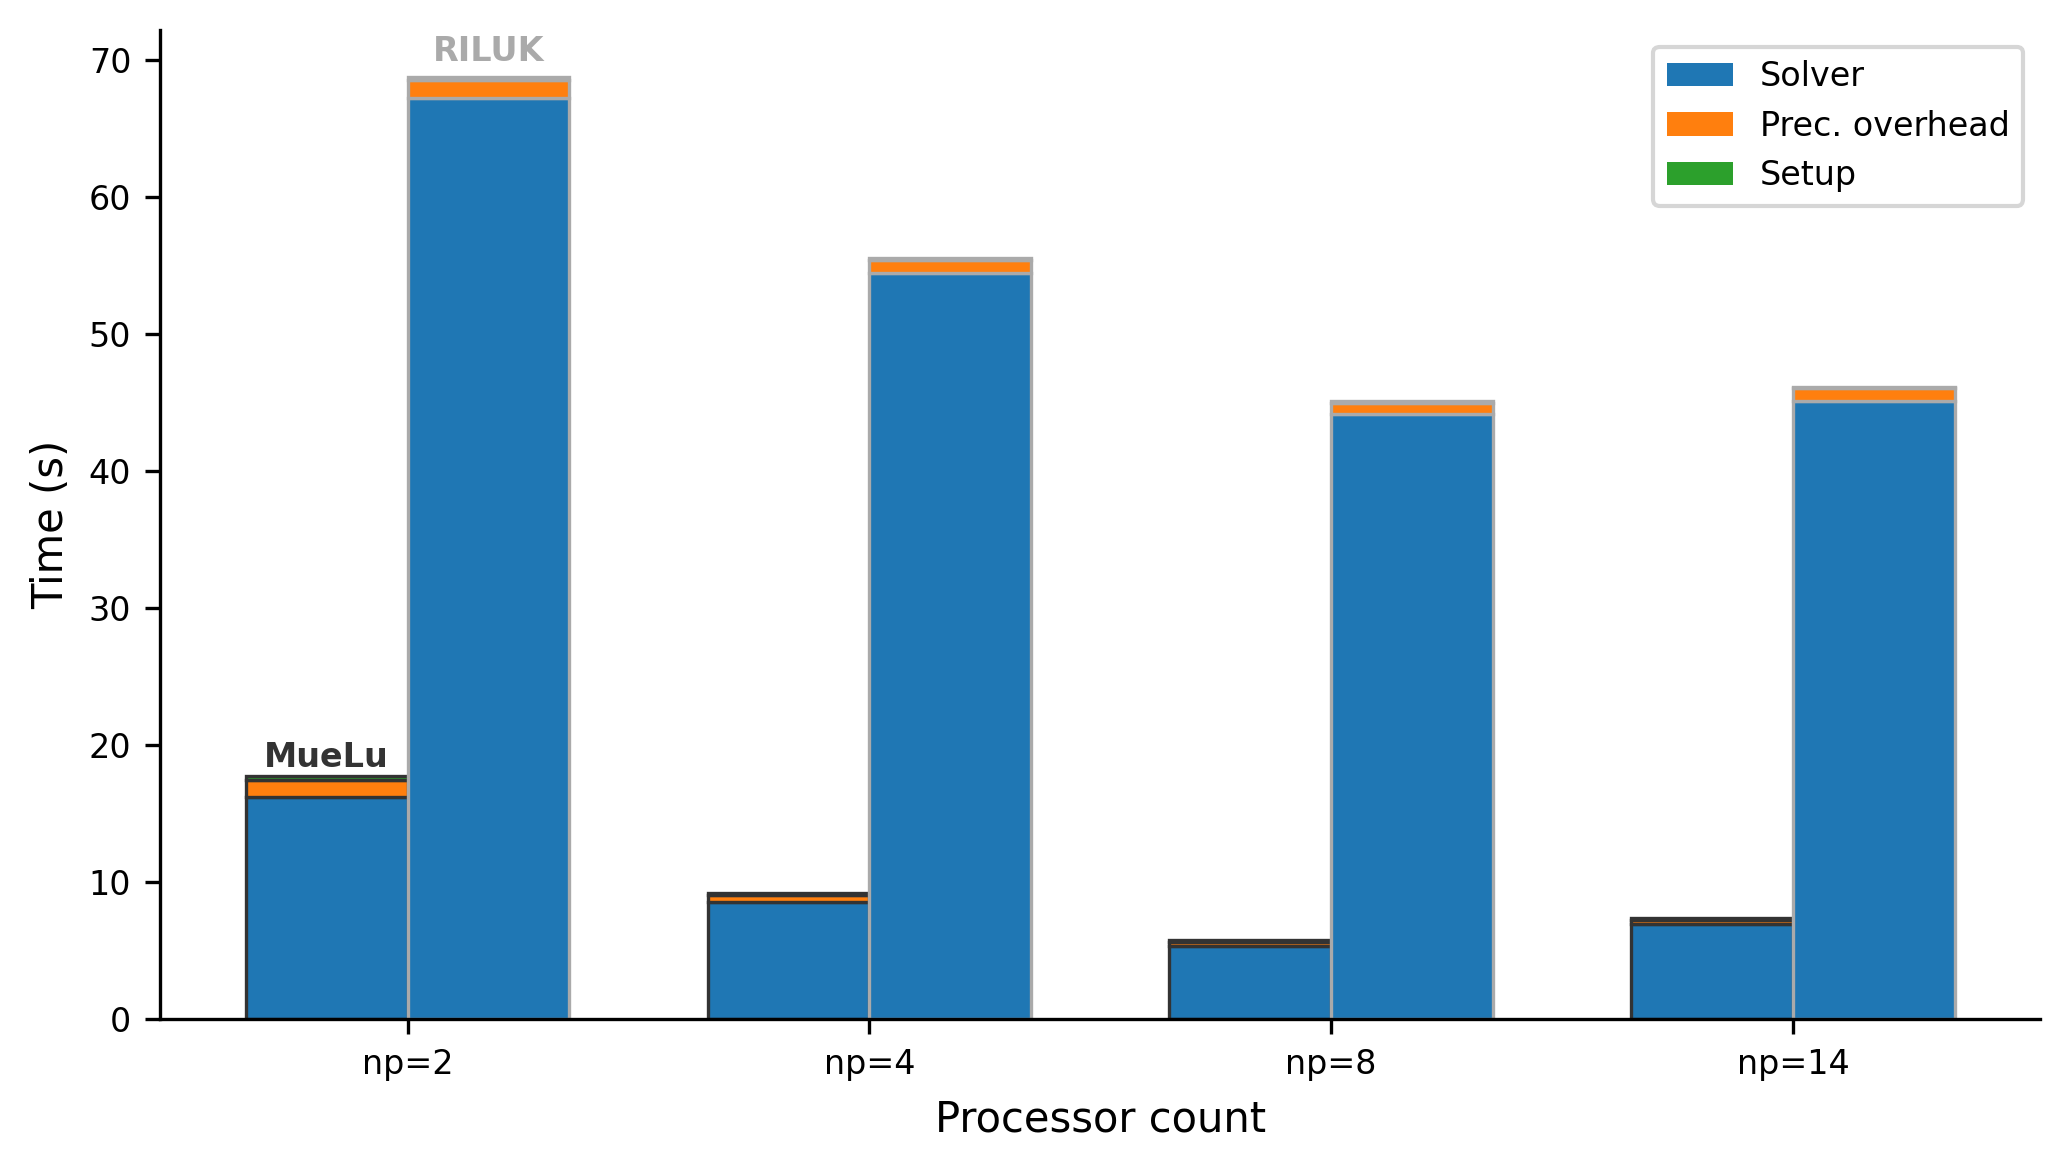
\includegraphics[width=0.9\textwidth]
	{../convergenceAnalysis/plotsAndData/optimalRun/time_breakdown.png}
	\caption{Time breakdown by section of the application. Setup involves reading the $\jR$ source and computing the conductivities. Preconditioner overhead displays the difference between the reported solve time by Belos and the wall clock time of the entire solve procedure. Solver is the reported solve time from Belos.}
	\label{fig:time_breakdown}
\end{figure}
\subsubsection{Summary}
While not a comprehensive analysis of the performance of this application, this study was used as a starting point to determine solver and preconditioner parameters. This provided a performance baseline that can be used to build and test the application. However, a more comprehensive study of solver runtime improvements is planned to be performed once the MHD interpolation is complete. The best performing MueLu-preconditioned GMRES configuration is used for all potential solves presented in Chapter~\ref{chap:results}.
